\documentclass[12pt]{article}
\usepackage[utf8]{inputenc}
\usepackage{amsmath,graphicx,psfrag,epsfig,graphicx,float,verbatim,spverbatim,listings,rotating,listings,multicol}

\setlength{\columnsep}{1cm}
\usepackage{circuitikz,tikz}
\usepackage[T1]{fontenc}
\usepackage{bigfoot} % to allow verbatim in footnote
\usepackage[numbered,framed]{matlab-prettifier}
\def\code#1{\texttt{#1}}
\usepackage{filecontents}
\usetikzlibrary{circuits.logic.US,circuits.logic.IEC}
\let\ph\mlplaceholder % shorter macro
\lstMakeShortInline"

\lstset{
  style              = Matlab-editor,
  basicstyle         = \mlttfamily,
  escapechar         = ",
  mlshowsectionrules = true,
}


\title{ExA}
\author{lmhg2 }
\date{Febuary 2019}

\begin{document}


\def\n{\noindent}
\def\u{\underline}
\def\hs{\hspace}
\newcommand{\thrfor}{.^{\displaystyle .} .}
\newcommand{\bvec}[1]{{\bf #1}}

\noindent
\rule{390pt}{0.5mm}

\begin{center}
{\bf ENGINEERING TRIPOS PART II A}
\end{center}
\vspace{0.5cm} {\bf GF2 \hfill SOFTWARE P2}
\vspace{0.5cm}
\begin{center}
{\bf INTERIM REPORT 1 - INTRODUCTION, GENERAL APPROACH, SYNTAX AND ERROR HANDLING \\
\hfill
\\Name: Group 7: Daniel Mackinnon, L\'ea Gansser-Potts \& Robbie Sewell\\\hfill\\
Colleges: Queens', Queens' \& Fitzwilliam\\\hfill\\
Report due: 18th May 2019 at 4pm
}
\end{center}
\rule{390pt}{0.5mm}

\newpage
\section{Introduction}
The aim of this project is to emulate a professional software development environment in which our team, made out of three software developers,  is tasked with designing and implementing an efficient logic circuit simulator package. This document outlines the structure put in place and the attitude adopted by the team to ensure that the challenges faced are overcome and a high quality product is delivered.  

\section{General Approach}
The general approach to the task is to keep the solutions simple and elegant. For instance, the grammar developed remains readable and as close to English as possible, all the while having a specific structure that allows for the parser's functions to be straightforward and robust. We aimed to complete a first iteration of the code within the first two weeks of the project, allowing time to build on this first draft as well as developing a intuitive, simple and straight-forward user interface, with features such as a `live parser' that would tell the user if they are making any syntactic or semantic errors as they input their circuit.\\

The user guide and the error handling mechanisms are being continuously added to as the software is developed in order to ensure that all bases have been covered, and no details missed.\\

As far as possible, the team has endeavoured to make collective and conscientious decisions at the start of the project regarding the language grammar and the timings that will allow for a simple implementation. \\

A modular approach has been adopted with the code, and specifically, the different functions in the \texttt{parser.py} module have been written by different team members. This was done in order for different solutions to similar problems to be found, and for the team to assess which solution is the most robust, before integrating and homogenising the software. Similarly, the GUI module will be done in a modular way, assigning the different features to individual team members, so that different approaches are considered and the most appropriate one followed. This modular approach has been adopted to easily spot where bugs in the program are, and for flexibility in the maintenance stage. 

\subsection{Teamwork planning}
The project has been divided into tasks, all of which have been given an `owner' and a `deadline'. The `owner' is responsible for understanding all the elements of the task and ensuring that it is delivered within the `deadline'. That being said, the task `owner' is not the only contributor to that task. A detail of the project schedule is given below: 

\begin{table}[H]
    \centering
    \begin{tabular}{||l|c|c||}
    \hline
          SUB TASK & OWNER & DEADLINE \\ [0.5ex]
          \hline \hline
         EBNF language & Dan & 16/05/19 \\
         Teamwork planning & L\'ea & 16/05/19 \\
         Error handling (syntatic and semantic) & Robbie & 16/05/19 \\
         Example circuit definition files x 2 & L\'ea & 18/05/19\\
         \hline
        \textbf{Interim report 1} & \textbf{L\'ea} & \textbf{18/05/19 at 4pm}\\ [0.5ex]
        \hline 
        \texttt{scanner.py} & Robbie & 18/05/19\\
        \texttt{names.py} & Robbie & 18/05/19\\
        Overall \texttt{parser.py} & Robbie & 20/05/19 \\
        \texttt{parser.py devices} function & Robbie & 20/05/19 \\
        \texttt{parser.py init} function & L\'ea & 20/05/19 \\
        \texttt{parser.py connections} function & Dan & 20/05/19 \\
        \texttt{parser.py monitor} function & Robbie & 20/05/19 \\
        Integration & Joint & 20/05/19\\
        \hline
        \multicolumn{2}{||l|}{GUI and pytests planning meeting} & Lab session 6 (20/05/19)\\
        \hline
        GUI & Robbie and Dan & 28/05/19 \\
        pytests & L\'ea & 28/05/19 \\
        User guide & Dan & 30/05/19 \\
        \hline
        \textbf{Interim report 2} & \textbf{Individual} & \textbf{30/05/19 at 11am}\\
        \hline
        Maintenance & tbc & 05/06/19\\
        \hline
       \textbf{Final report} & \textbf{Individual} & \textbf{05/06/19 at 4pm}\\
        \hline \hline
        
    \end{tabular}
    \caption{Work schedule}
    \label{tab:schedule}
\end{table}

Full planning of the GUI module and the pytest have not been undertaken at this point, the schedule will be completed after the planning meeting scheduled for the 20/05/19. 

Furthermore \textit{git} has been used to track the contribution of the different teams members, but only the software has been included on the shared repository, which can be found at \texttt{https://github.com/rsewell97/GF2-Software}.

 
\section{EBNF for syntax}

The attitude adopted was to keep the \texttt{.txt} file as readable and flexible as possible, while keeping the language straightforward to interpret by the parser. 
\\
The description file contains four main sections:
\begin{itemize}
\item “\textit{Devices}”: where the digital devices are listed.  Certain devices have the optional argument of the number of inputs to it which may also be specified. Error handling has been implemented to ensure that an appropriate number of inputs for each different gate type is respected. 
\item “\textit{Init}”: where switches and a clock signal are initialised. All switches default to a \texttt{False} boolean value unless otherwise specified.
\item “\textit{Connections}”: The wiring from outputs to inputs of devices. Each device may appear in any order. The inputs can be specified in any order.   
\item “\textit{Monitor}”: An optional section containing a list of the outputs of devices which should be displayed to the user. If this section is not included, the outputs of all devices will be shown to the user
\end{itemize}

Below is the grammar developed for our encryption language:

\begin{spverbatim}
device_name =  letter, {letter | digit}

port_name =  digit, [digit] 

devices_type = “DTYPE” | “NAND” | “NOR” | “XOR” | “AND” | “OR” | “CLOCK” | “SWITCH”

connection = “to”

definition = “is” | “are”

possession = “has” | “have”

curly_open = “{“

curly_closed = “}”

dot =  “.”

comma = “,”

arrow = (“=>” | “->”)

colon = “:”

range = device_name, arrow, device_name

device_definition = (device_name, {comma , device_name} | range), definition, (device_type)

device_specification = (name, {comma , name} | range), possession, number

switch_level = “set” , (device_name, {comma , device_name} | range) , (“HIGH” | “LOW”)

clock_initialiser = (name, {comma , name} | range), "has" ,“cycle", ["time of"], number

connect_definition = device_name, [“BAR”], connection, device_name, dot, port_name

full_device_name = “Device”, name

device_connection_definition = full_device_name , [colon] , curly_open, connect_definition, {connect_definition}, curly_close

whole_devices = (“devices” | “Devices”| "DEVICES"), [colon], curly_open, device_definition, {device_definition}, device_specification, {device_specification}, curly_close

whole_init = (“init” | “Init” | "INIT"), [colon], curly_open, device_definition, {device_definition}, {clock_initailiser | switch_level}, {device_definition}, {clock_initailiser | switch_level}, curly_close

whole_connections = (“connections” | “Connections” |"CONNECTIONS"), [colon], curly_open, device_connection_definition, {device_connection_definition}, curly_close

whole_monitor = (“monitor” | “Monitor” | "MONITOR"), [colon], curly_open, (name {comma, name} | range), {name {comma, name} | range}, curly_close

entirety = whole_devices, whole_init, whole_connections, whole_monitor

\end{spverbatim}

Notes on the language definition:
\begin{itemize}
\item The language treats \texttt{init} and \texttt{device} definitions identically, but these are distinct in the the parser. 
\item Colons after a heading and before the opening of a curly bracket can be used to improve readability, but the language does not require them. 
\item It is expected that the language definition will be revised as the implementation of the software is undertaken.  
\item Tabs-breaks are not considered part of the syntax of the definition file. The order of appearance of each section is important when parsing the language.
\item  Both “devices” and “inputs” must appear ahead of “connections”. In addition, “devices” must appear before “monitor”.
\item Curly brackets {} are used to delimit the different sections and nest subsections within a section. This will be useful in the implementation as they can be used 'checkpoints' during error handling.  

\end{itemize}

To illustrate the EBNF detailed, two examples have been provided with their circuit diagrams. 

\subsection{Example A - Simple circuit}

\begin{figure} [ht]
\begin{center}
\fbox{
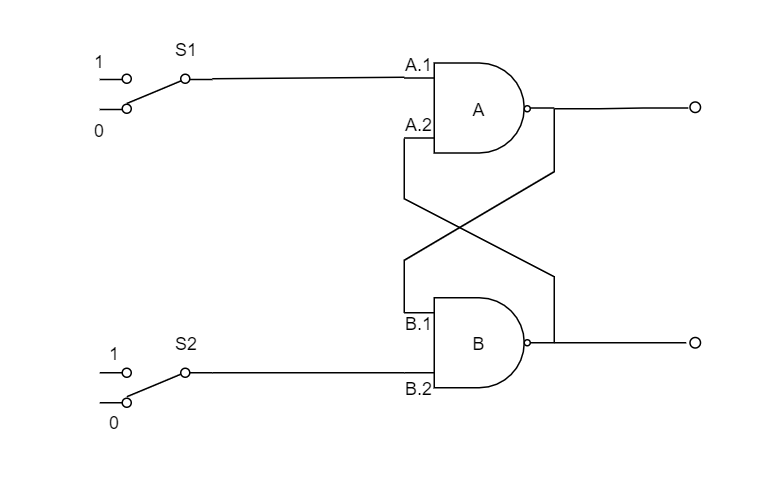
\includegraphics[width = 0.8\linewidth]{simple.png}
}
\caption{SR flip flip circuit}
\label{fig1:SR flip flip circuit}
\end{center}
\end{figure}

The code that defines the circuit in figure \ref{fig1:SR flip flip circuit} is given by:


\begin{minipage}{\linewidth}
\begin{lstlisting}
devices: {
    A,B are NAND gates
    A, B have 2 inputs
}
init: {
    S1, S2 are switches
    set S1, S2 low
}
connections: {
    device A: {
        S1 to A.1
        B to A.2
    }
    device B: {
        A to B.1
        S2 to B.2
    }
}
monitor: {
    A, B
}
\end{lstlisting}
\end{minipage}

\subsection{Example B - Complex circuit}
 \begin{figure} [ht]
\begin{center}
\fbox{
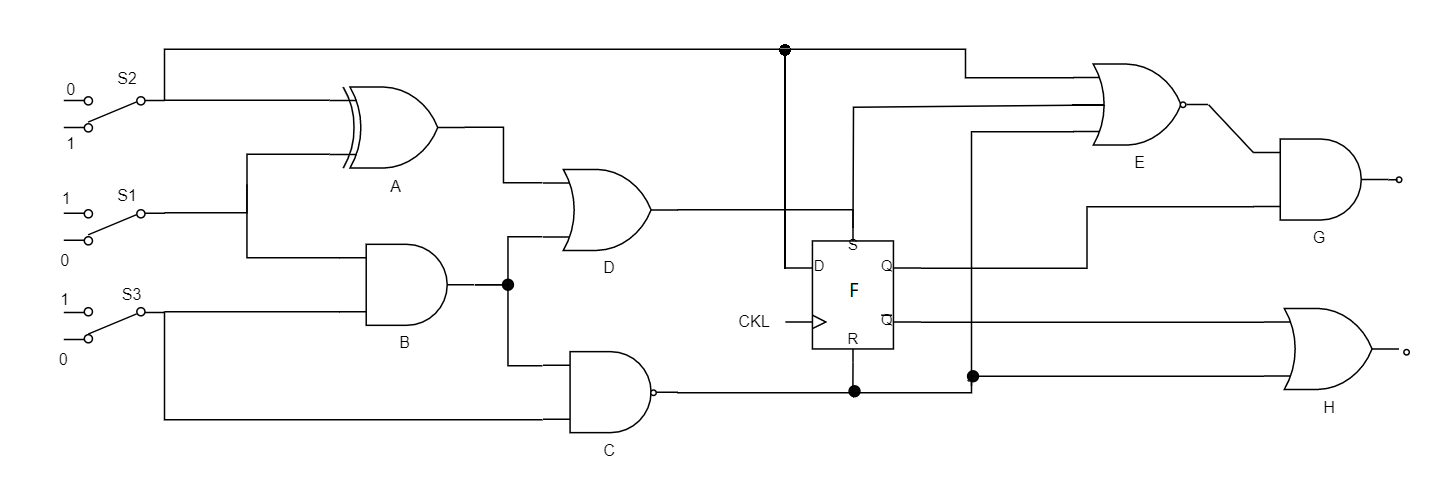
\includegraphics[width = \linewidth]{complex.PNG}
}
\caption{Trivial complex circuit}
\label{fig2:trivial complex circuit}
\end{center}
\end{figure}

The logic circuit described in the figure \ref{fig2:trivial complex circuit} is trivial, and was constructed as an exercise to test the grammar rules of the language. Input gate names have been omitted for clarity, but it is noteworthy that which way round the inputs are do not matter other than for a D-type date, in which case the inputs are defined below, for a device named F: \\
\begin{center}
\begin{tabular}{|c c|}
\hline 
    Name & Gate\\
    \hline  
    F.CLK & CLOCK\\
    F.SET & SET \\
    F.CLEAR & CLEAR\\
    F.DATA & DATA  \\
    \hline 
\end{tabular}
\end{center}


The definition file for the circuit can be found below:
\pagebreak


\begin{multicols}{2}
\begin{lstlisting}
Devices: {
    A is an XOR gate
    B is a AND gate
    C is a NAND gate
    D is an OR gate
    E is NOR gate
    F is a DTYPE
    G is NAND
    H is OR
    A,B,C,D,G,H have 2 inputs
    E has 3 inputs
}

Init: {
    S1 => S3 are SWITCH inputs
    set S2 high
    CKL1 is a CLOCK input
    CKL1 has cycle time of 5
}

Connections: {
    Device A: {
        S2 to A.1
        S3 to A.2
    }
    Device B: {
        S1 to B.1
        S3 to B.2
    }
    Device C: {
        B to C.1
        S3 to C.2
    }
    Device D: {
        A to D.1
        B to D.2
    }
    Device E: {
        S2 to E.1
        D to E.2
        C to E.3
    }
    Device F: {
        CLK1 to F.CLK
        D to F.SET
        C to F.CLEAR
        S2 to F.DATA
    }
    Device G: {
        E to G.1
        F to G.2
    }
    Device H: {
        FBAR to H.1 
        C to H.2
    }
}

Monitor: {
    B, G, H
} 
\end{lstlisting}
\end{multicols}

% \begin{tikzpicture}[minimum height=0.75cm] 
%     \node[and gate US, draw,logic gate inputs=nnn] (A) {}; 
%     \foreach \a in {1,...,3}
%         \draw (A.input \a -| -1,0) -- (A.input \a); 
%     \draw (A.output) -- ([xshift=0.5cm]A.output);
% \end{tikzpicture}   

\subsection{Error Identification and handling}

Error identification is a key aspect of a user-friendly program. Therefore, there are several ways in which errors have been handled:
\begin{itemize}
\item Errors are raised immediately as the parser encounters them in the definition file.
\item A useful message describing the nature and location (displaying the erroneous line, with a cursor indicating the point that the parser has failed) will be displayed to the user. This has been treated in a separate \texttt{error.py} module.
\item Hints with what is expected in the error's location will be given.
\item As the software is being developed, whenever the code makes an assumption, an error will be thrown. 
\end{itemize}
\hline
\end{document}